\documentclass{article}

% if you need to pass options to natbib, use, e.g.:
%     \PassOptionsToPackage{numbers, compress}{natbib}
% before loading neurips_2022

% ready for submission
\usepackage[preprint]{neurips_2022}

% to compile a preprint version, e.g., for submission to arXiv, add add the
% [preprint] option:
%     \usepackage[preprint]{neurips_2020}

% to compile a camera-ready version, add the [final] option, e.g.:
%     \usepackage[final]{neurips_2020}

% to avoid loading the natbib package, add option nonatbib:
%\usepackage[nonatbib]{neurips_2020}
\usepackage[utf8]{inputenc} % allow utf-8 input
\usepackage[T1]{fontenc}    % use 8-bit T1 fonts
\usepackage{hyperref}       % hyperlinks
\usepackage{url}            % simple URL typesetting
\usepackage{booktabs}       % professional-quality tables
\usepackage{amsfonts}       % blackboard math symbols
\usepackage{nicefrac}       % compact symbols for 1/2, etc.
\usepackage{microtype}      % microtypography


% Graphics and color
\usepackage{graphicx}
\usepackage{xcolor}

% References and Bibliography
\usepackage{url}
\usepackage{hyperref}
\hypersetup{
  colorlinks,
  linkcolor={black},
  citecolor={blue!50!black},
  urlcolor={blue!50!black}
}
\usepackage{cleveref}
\usepackage[numbered]{bookmark} % Fixes false PDF table of contents
\usepackage{natbib}
\setcitestyle{numbers,sort&compress,square,comma}
\usepackage{bibentry}
\nobibliography*

\title{Impact of most Common Food Categories on\\ Green House Gas Emissions}


\author{%
  Hanna Dettki\thanks{Equal contribution.} \\
  Department of Computer Science\\
  University of Tübingen\\
  \texttt{hanna.dettki@student.uni-tuebingen.de} \\
  \And
  Davide $^{*}$  \\
  Department of Computer Science\\
  University of Tübingen\\
  \texttt{@student.uni-tuebingen.de} \\
  % \AND
  % Coauthor \\
  % Affiliation \\
  % Address \\
  % \texttt{email} \\
  % \And
  % Coauthor \\
  % Affiliation \\
  % Address \\
  % \texttt{email} \\
  % \And
  % Coauthor \\
  % Affiliation \\
  % Address \\
  % \texttt{email} \\
}

\begin{document}

\maketitle

\begin{abstract}
  This research is made for the Data Literacy Project of the academic year 2022/2023. It covers the discussion about the emissions of a plant based diet in comparison with a traditional diet. The research is conducted by exploration of the data, hypothesis testing and example comparisons. 
\end{abstract}

\section{Introduction}




\subsection{Research Question}



\section{Data}
\label{data}

\paragraph{Handling missing data}
We substituted  missing  data by taking the mean of the respecting feature. 
\subsection{Data Generating Process}
\label{dataGen}



\section{Analysis}
\label{analysis}


\begin{figure}[h]
  \centering
  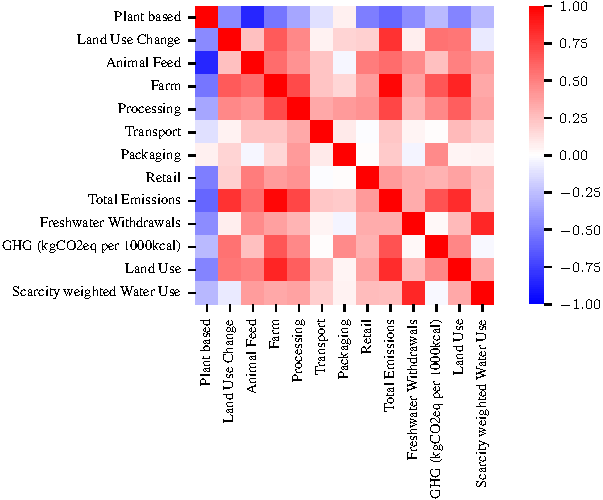
\includegraphics[width=0.75\textwidth]{figures/heat-map.pdf}
  \caption{Some caption text.}
\end{figure}

\subsection{Average Emissions for Plant-based and Animal-based Products}
\paragraph{Eutrophying emissions}
\paragraph{Accounting  for Nutritional Value}
\paragraph{Comparing Typical Diets}

\section{Conclusion}
\label{conclusion}


\section{Limitations}
\label{limitations}

\subsection{Citations within the text}


\subsection{Tables}



Note that publication-quality tables \emph{do not contain vertical rules.} We
strongly suggest the use of the \verb+booktabs+ package, which allows for
typesetting high-quality, professional tables:
\begin{center}
  \url{https://www.ctan.org/pkg/booktabs}
\end{center}
This package was used to typeset Table~\ref{sample-table}.

\begin{table}
  \caption{Sample table title}
  \label{sample-table}
  \centering
  \begin{tabular}{lll}
    \toprule
    \multicolumn{2}{c}{Part}                   \\
    \cmidrule(r){1-2}
    Name     & Description     & Size ($\mu$m) \\
    \midrule
    Dendrite & Input terminal  & $\sim$100     \\
    Axon     & Output terminal & $\sim$10      \\
    Soma     & Cell body       & up to $10^6$  \\
    \bottomrule
  \end{tabular}
\end{table}


\section*{Broader Impact}

\begin{itemize}
\item reducing GHG
\item animal welfare
\item biodiversity
\item Health: While there are some concerns, that vegan diets (i.e, plant-based diets that exclude all forms of animal products in their entirety) are not sufficient w.r.t providing recommended micronutiernt levels (e.g. vitamin B12, zinc, iron, etc.), they generally meet protein intake recommendations. Nonetheless, individuals who consume a vegan diet should remain aware regarding potential micronutirent insufficiencies. 
\end{itemize}



\section*{Literature}

List of selected central research literature that the project is based on.


\begin{itemize}
  \item \bibentry{Ritchie2020}
  \item \bibentry{Michigan2021}
  \item test \citet{WHO2021}
\end{itemize}

\subsection{Related Literature}
\begin{itemize}
  \item \bibentry{Pieper2020}
  %\item \bibentry{Felix2021}
\end{itemize}


{\small
\bibliographystyle{unsrtnat}
\bibliography{../literature/references.bib}
}
\end{document}
